
\documentclass[border=10pt, 12pt]{standalone}
\usepackage[svgnames]{xcolor}
\usepackage{amsmath}
\usepackage{pgfplots}
\pgfplotsset{compat=newest}
\usepackage[sfdefault]{FiraSans}
\usepackage{FiraMono}
\renewcommand*\familydefault{\sfdefault}
\begin{document}
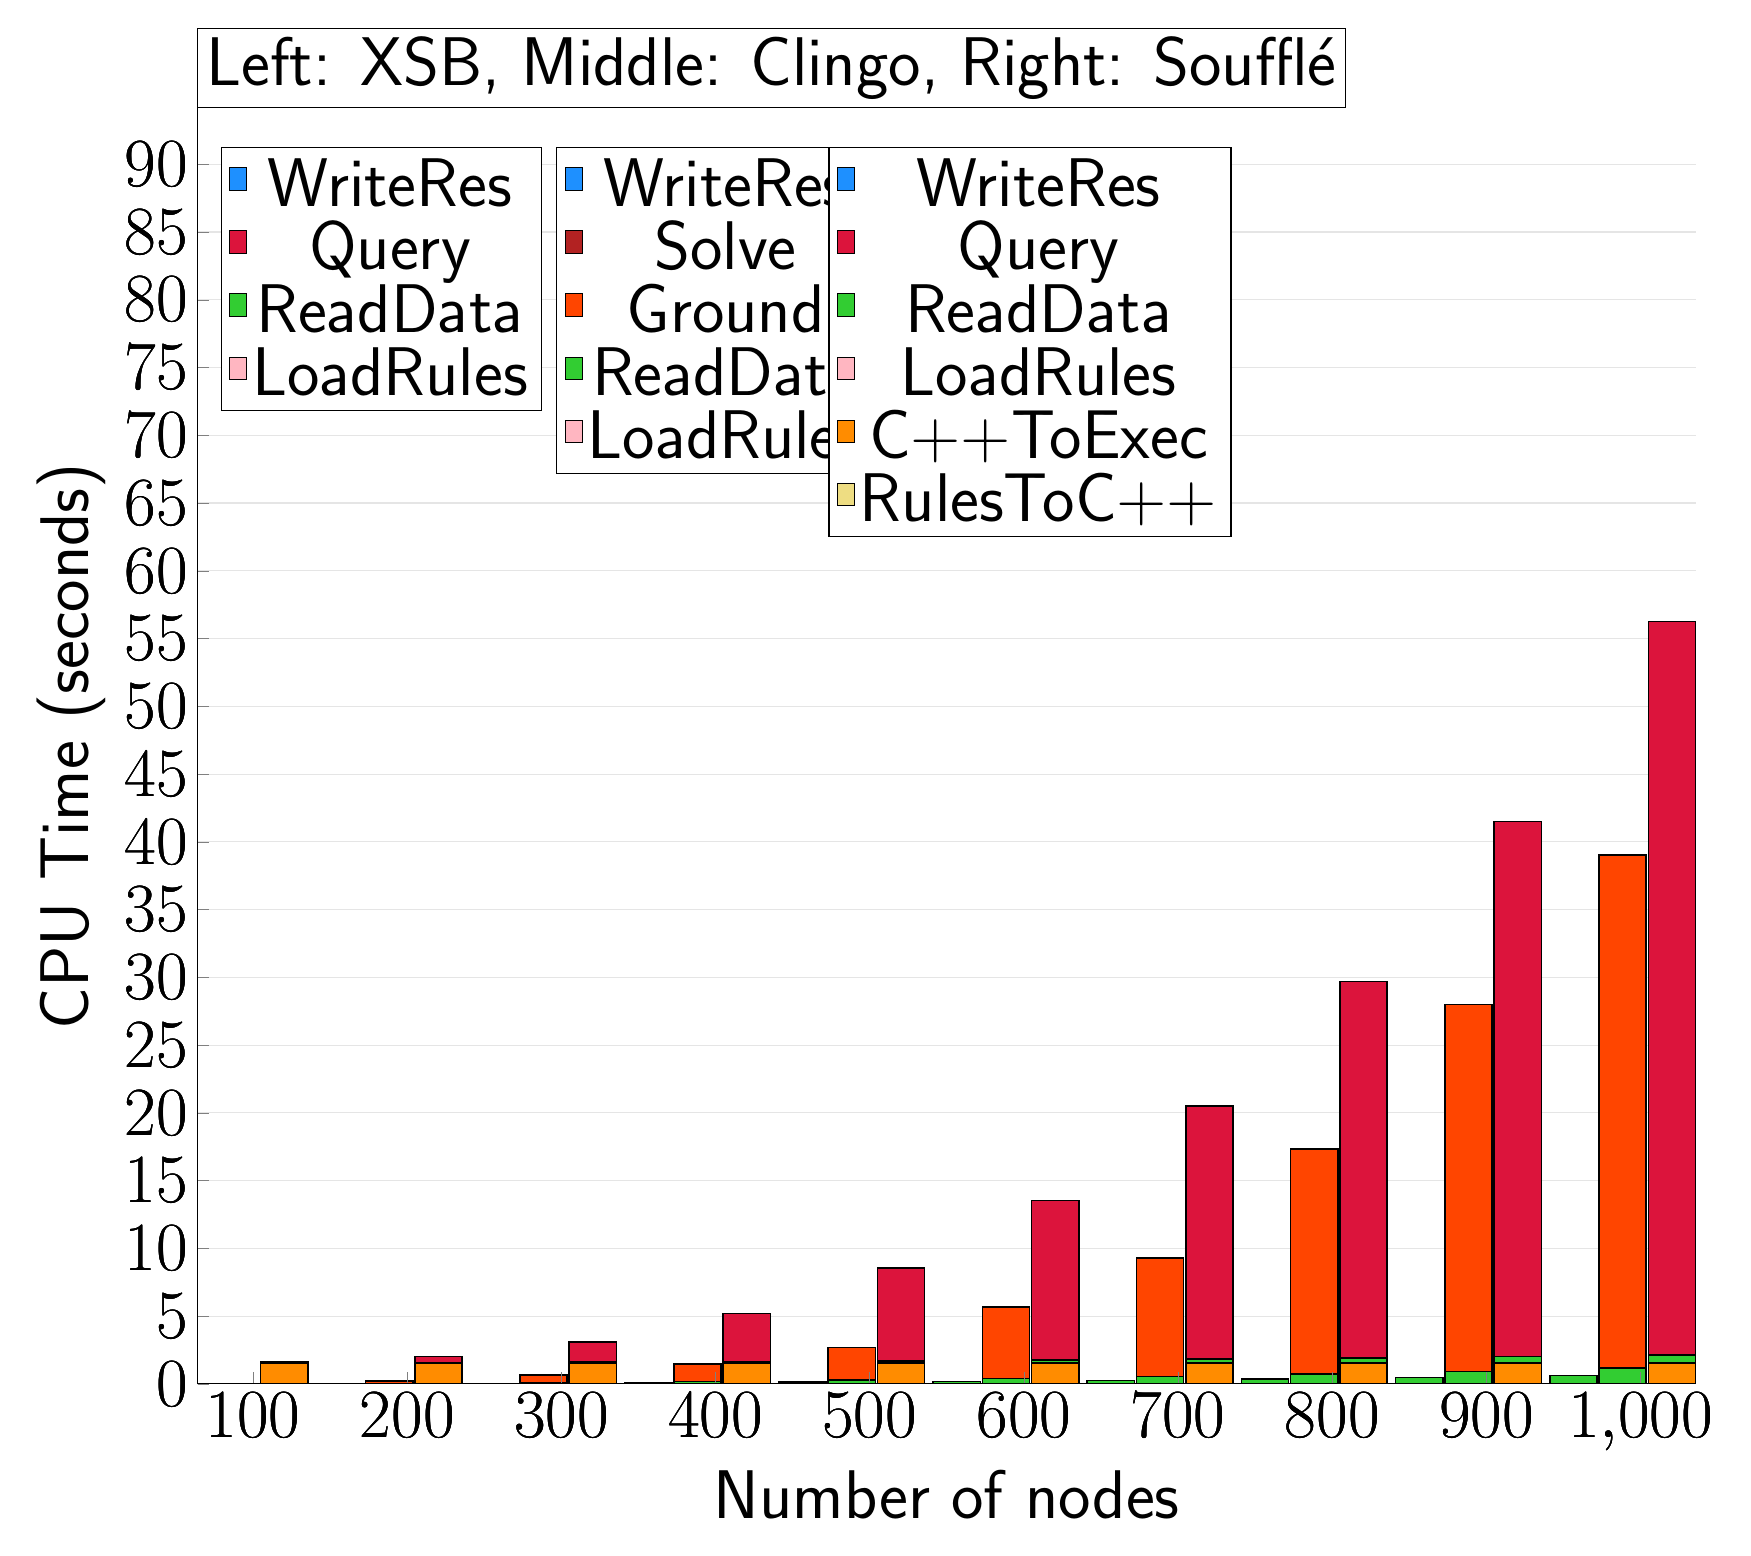
\begin{tikzpicture}
                        \begin{axis}[bar shift=-24.3pt, 
   ybar stacked,
   width=1.7\textwidth,
   bar width=0.6cm,
   ymajorgrids, tick align=inside,
   major grid style={draw=gray!20},
   xtick=data,
   ymin=0, ymax=94.12288,
   axis x line*=bottom,
   axis y line*=left,
   enlarge x limits=0.04,
   legend style={
       at={(0.23, 0.97)},
       anchor=north east,
       legend columns=1,
       font=\Huge,
   },
   ylabel={CPU Time (seconds)},
   xlabel={Number of nodes},
   label style={font=\Huge},
   tick label style={font=\Huge},
]
\addlegendimage{fill=DodgerBlue, draw=black, line width=0.2pt}
\addlegendentry{WriteRes}
\addlegendimage{fill=Crimson, draw=black, line width=0.2pt}
\addlegendentry{Query}
\addlegendimage{fill=LimeGreen, draw=black, line width=0.2pt}
\addlegendentry{ReadData}
\addlegendimage{fill=LightPink, draw=black, line width=0.2pt}
\addlegendentry{LoadRules}
\addplot +[fill=LightPink, draw=black, line width=0.55pt] coordinates {
(100, 0.0005514000000000001)
(200, 0.0005558000000000001)
(300, 0.0005594000000000003)
(400, 0.0005540000000000005)
(500, 0.0005610000000000003)
(600, 0.0005526000000000002)
(700, 0.0005542000000000002)
(800, 0.0005553999999999996)
(900, 0.0005540000000000005)
(1000, 0.0005562)
};
\addplot +[fill=LimeGreen, draw=black, line width=0.55pt] coordinates {
(100, 0.004052600000000001)
(200, 0.0170224)
(300, 0.039853000000000006)
(400, 0.0747092)
(500, 0.12197100000000001)
(600, 0.18372899999999998)
(700, 0.2592078)
(800, 0.35407939999999993)
(900, 0.46937059999999997)
(1000, 0.6065582)
};
\addplot +[fill=Crimson, draw=black, line width=0.55pt] coordinates {
(100, 3.6000000000001303e-06)
(200, 4.599999999999048e-06)
(300, 4.599999999999048e-06)
(400, 5.800000000003024e-06)
(500, 6.399999999989743e-06)
(600, 7.000000000001449e-06)
(700, 6.59999999998995e-06)
(800, 6.600000000001052e-06)
(900, 6.599999999989949e-06)
(1000, 6.800000000017904e-06)
};
\addplot +[fill=DodgerBlue, draw=black, line width=0.55pt] coordinates {
(100, 6.0400000000000384e-05)
(200, 6.0200000000000555e-05)
(300, 6.080000000000255e-05)
(400, 6.19999999999926e-05)
(500, 6.260000000000708e-05)
(600, 6.459999999999797e-05)
(700, 6.520000000000966e-05)
(800, 6.580000000000472e-05)
(900, 6.56000000000323e-05)
(1000, 6.659999999998335e-05)
};
\end{axis}

\begin{axis}[bar shift=-6.5pt, 
   ybar stacked,
   width=1.7\textwidth,
   bar width=0.6cm,
   ymajorgrids, tick align=inside,
   major grid style={draw=none},
   xtick=data,
   ymin=0, ymax=94.12288,
   axis x line*=none,
   axis y line*=none,
   enlarge x limits=0.04,
   legend style={
       at={(0.454, 0.97)},
       anchor=north east,
       legend columns=1,
       font=\Huge,
   },
   label style={font=\Huge},
   tick label style={font=\Huge},
]
\addlegendimage{fill=DodgerBlue, draw=black, line width=0.2pt}
\addlegendentry{WriteRes}
\addlegendimage{fill=FireBrick, draw=black, line width=0.2pt}
\addlegendentry{Solve}
\addlegendimage{fill=OrangeRed, draw=black, line width=0.2pt}
\addlegendentry{Ground}
\addlegendimage{fill=LimeGreen, draw=black, line width=0.2pt}
\addlegendentry{ReadData}
\addlegendimage{fill=LightPink, draw=black, line width=0.2pt}
\addlegendentry{LoadRules}
\addplot +[fill=LightPink, draw=black, line width=0.55pt] coordinates {
(100, 0.0)
(200, 0.0)
(300, 0.0)
(400, 0.0)
(500, 0.0)
(600, 0.0)
(700, 0.0)
(800, 0.0)
(900, 0.0)
(1000, 0.0)
};
\addplot +[fill=LimeGreen, draw=black, line width=0.55pt] coordinates {
(100, 0.010000000000000009)
(200, 0.040000000000000036)
(300, 0.09600000000000003)
(400, 0.16999999999999998)
(500, 0.272)
(600, 0.396)
(700, 0.542)
(800, 0.714)
(900, 0.8979999999999999)
(1000, 1.1620000000000001)
};
\addplot +[fill=OrangeRed, draw=black, line width=0.55pt] coordinates {
(100, 0.020000000000000018)
(200, 0.15799999999999997)
(300, 0.5600000000000002)
(400, 1.296)
(500, 2.4160000000000004)
(600, 5.2780000000000005)
(700, 8.73)
(800, 16.624000000000002)
(900, 27.096000000000004)
(1000, 37.858)
};
\addplot +[fill=FireBrick, draw=black, line width=0.55pt] coordinates {
(100, 0.0)
(200, 0.0)
(300, 0.0)
(400, 0.0020000000000000018)
(500, 0.0)
(600, 0.00400000000000027)
(700, 0.0019999999999999575)
(800, 0.005999999999999517)
(900, 0.001999999999999602)
(1000, 0.005999999999998807)
};
\addplot +[fill=DodgerBlue, draw=black, line width=0.55pt] coordinates {
(100, 0.0)
(200, 0.0)
(300, 0.0)
(400, -0.0020000000000000018)
(500, 0.0)
(600, -0.00400000000000027)
(700, -0.0019999999999999575)
(800, -0.005999999999999517)
(900, -0.001999999999999602)
(1000, -0.005999999999998807)
};
\end{axis}

\begin{axis}[bar shift=11.3pt, 
   ybar stacked,
   width=1.7\textwidth,
   bar width=0.6cm,
   ymajorgrids, tick align=inside,
   major grid style={draw=none},
   xtick=data,
   ymin=0, ymax=94.12288,
   axis x line*=none,
   axis y line*=none,
   enlarge x limits=0.04,
   legend style={
       at={(0.69, 0.97)},
       anchor=north east,
       legend columns=1,
       font=\Huge,
   },
   label style={font=\Huge},
   tick label style={font=\Huge},
]
\addlegendimage{fill=DodgerBlue, draw=black, line width=0.2pt}
\addlegendentry{WriteRes}
\addlegendimage{fill=Crimson, draw=black, line width=0.2pt}
\addlegendentry{Query}
\addlegendimage{fill=LimeGreen, draw=black, line width=0.2pt}
\addlegendentry{ReadData}
\addlegendimage{fill=LightPink, draw=black, line width=0.2pt}
\addlegendentry{LoadRules}
\addlegendimage{fill=DarkOrange, draw=black, line width=0.2pt}
\addlegendentry{C++ToExec}
\addlegendimage{fill=LightGoldenrod, draw=black, line width=0.2pt}
\addlegendentry{RulesToC++}
\addplot +[fill=LightGoldenrod, draw=black, line width=0.55pt] coordinates {
(100, 0.010000000000000002)
(200, 0.006000000000000001)
(300, 0.0020000000000000005)
(400, 0.008000000000000002)
(500, 0.010000000000000002)
(600, 0.004000000000000001)
(700, 0.008000000000000002)
(800, 0.004000000000000001)
(900, 0.0020000000000000005)
(1000, 0.008000000000000002)
};
\addplot +[fill=DarkOrange, draw=black, line width=0.55pt] coordinates {
(100, 1.5320000000000003)
(200, 1.532)
(300, 1.53)
(400, 1.534)
(500, 1.5260000000000002)
(600, 1.532)
(700, 1.532)
(800, 1.5240000000000002)
(900, 1.536)
(1000, 1.5219999999999998)
};
\addplot +[fill=LightPink, draw=black, line width=0.55pt] coordinates {
(100, 0.0001602)
(200, 0.0001594)
(300, 0.00015759999999999998)
(400, 0.00016079999999999998)
(500, 0.0001564)
(600, 0.0001674)
(700, 0.0001692)
(800, 0.00015500000000000003)
(900, 0.0001712)
(1000, 0.00016619999999999997)
};
\addplot +[fill=LimeGreen, draw=black, line width=0.55pt] coordinates {
(100, 0.013366)
(200, 0.040089)
(300, 0.07362099999999999)
(400, 0.11325959999999999)
(500, 0.1603278)
(600, 0.22786040000000002)
(700, 0.30169320000000005)
(800, 0.38707)
(900, 0.48928720000000003)
(1000, 0.5972678)
};
\addplot +[fill=Crimson, draw=black, line width=0.55pt] coordinates {
(100, 0.0728016)
(200, 0.45096179999999997)
(300, 1.49461)
(400, 3.518956)
(500, 6.835151999999999)
(600, 11.76698)
(700, 18.64922)
(800, 27.7854)
(900, 39.488519999999994)
(1000, 54.122879999999995)
};
\addplot +[fill=DodgerBlue, draw=black, line width=0.55pt] coordinates {
(100, 7.04e-05)
(200, 0.00013719999999999997)
(300, 0.000125)
(400, 0.0001632)
(500, 0.0001808)
(600, 0.0001642)
(700, 0.00018240000000000002)
(800, 0.0001754)
(900, 0.0002398)
(1000, 0.00016380000000000002)
};
\end{axis}


\node[anchor=south, draw, fill=white] at (rel axis cs:0.42,1) {\Huge Left: XSB, Middle: Clingo, Right: Soufflé};
\end{tikzpicture}
\end{document}
                    